% Drawing 154/08-23 -- folder 154, batch 08, archive page 153 (PDF page 154).
% Transcription: en bas, trois dessins : une étoile de trois droites au crayon, l'une fléchée ; la projection d'un cube (hexagone à sommets marqués) entourée de deux ellipses brunes ; un cercle portant huit petites marques
% Kind: star of three lines; cube projection in two ellipses; circle with eight marks. Method 2 (schematic redraw from the facsimile). Status: ok.
% Notes: Star: three pencil strokes through one point, the nearly horizontal one ending in an arrowhead. Redrawn 2026-11-12 (issue 128): to check again. 2026-11-14, Claude Opus 5.5, overlay check (issue 147): rasterised from its own coordinates over the 400 dpi colour scan (402 ppi native) on a unit grid; not compiled (no TeX in the session). The three figures, read from a page view, lay 1 to 5 units off their ink (the circle's ticks at the compass points, an inner vertex of the cube that the page does not have) and are redrawn on crops at 19 to 40 px per unit. Star: three pencil strokes crossing near one point, the nearly horizontal one arrowed, the other two doubled on the page. Cube: a closed black outline through seven black dots and a brown blob (on the right, where the tilted ellipse crosses it), the bottom stroke stopping short of the lower dot as on the page; no inner vertex or inner edge is drawn on the page; the left dot of the lower pair is ringed in brown; two brown ellipses round it, the upright one open on its right where the tilted one crosses, the tilted one ending at the lower left in a short hook; two short brown dashes inside. Circle: a thick black circle (its top just above the crop) with six short ticks across the rim, at the top, upper left, upper right, left, lower right and bottom, and two stretches of the rim drawn over (at the left and at the lower left), which may be the remaining two of the transcription's eight marks. Laid over the scan again, every stroke lies on its ink to within about 0.5 unit. Status set to ok.
% Coordinates: 1 unit = 1 mm = 1/100 of the crop width (bbox in page fractions: [0.365, 0.42, 0.79, 0.52]).
% Redrawn by Claude (claude-fable-5-2), issue #128, 2026-11-12; not checked by a human; not compiled (no TeX in the session).
% Checked by Claude (claude-opus-5-5) 2026-11-14 (issue #147): overlaid on the 400 dpi colour facsimile; not compiled (no TeX in the session). Not checked by a human. Status: ok.
% Rights: reproduces part of the work -- behind RENDER_TRANSCRIPTS, never published by itself.
\documentclass[tikz,border=3pt]{standalone}
\usepackage{amsmath,amssymb}
\usetikzlibrary{patterns,arrows.meta}
\tikzset{Br/.style={brown!80!black}, pencil/.style={black!45}, struck/.style={black!35}, mpt/.style={circle,draw,inner sep=1.3pt}, pt/.style={circle,fill,inner sep=0.9pt}, opt/.style={circle,draw,fill=white,inner sep=1.1pt}}
\begin{document}
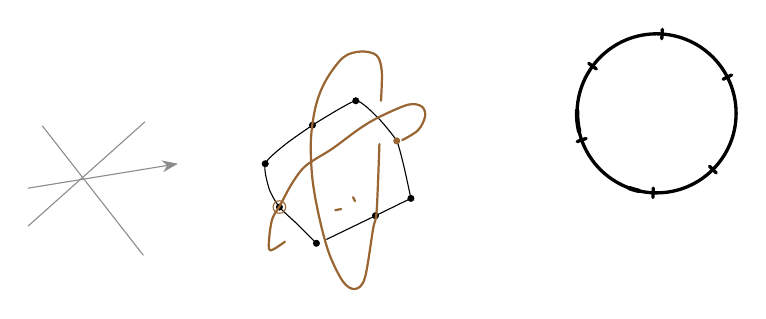
\begin{tikzpicture}[x=1mm,y=1mm,line cap=round,line join=round,font=\scriptsize]
\draw[pencil,-{Stealth[length=2mm]}] (0,-18.6) -- (19,-15.5);
\draw[pencil] (1.8,-10.7) -- (14.6,-27.1);
\draw[pencil] (14.8,-10.2) -- (0,-23.4);
\draw plot[smooth, tension=0.3] coordinates {(36.1,-10.6) (41.6,-7.5) (44.5,-9.75) (46.8,-12.6) (47.75,-16) (48.6,-19.9)};
\draw (48.6,-19.9) -- (44.1,-22.1) -- (37.9,-25.1);
\draw plot[smooth, tension=0.4] coordinates {(36.6,-25.6) (34.2,-23.2) (31.9,-21) (30.6,-18.7) (30.1,-15.5) (32.7,-13) (36.1,-10.6)};
\node[pt] at (41.6,-7.5) {};
\node[pt] at (36.1,-10.6) {};
\node[pt] at (30.1,-15.5) {};
\node[pt] at (31.9,-21) {};
\node[pt] at (36.6,-25.6) {};
\node[pt] at (44.1,-22.1) {};
\node[pt] at (48.6,-19.9) {};
\node[pt,Br] at (46.8,-12.6) {};
\draw[Br] (31.9,-21) circle[radius=0.8];
\draw[Br,thick] plot[smooth, tension=0.55] coordinates {(32.6,-25.4) (30.75,-26.5) (30.6,-25) (31,-22.5) (32,-20.75) (33.5,-18) (35.25,-15.75) (38.6,-13.6) (42,-11.1) (44.5,-9.6) (48.25,-8) (50,-8.25) (50.4,-9.5) (49.5,-11.25) (47.5,-12.5)};
\draw[Br,thick] plot[smooth, tension=0.55] coordinates {(44.6,-13) (44.25,-21.5) (43.8,-23.75) (42.75,-30) (41.5,-31.4) (40,-30.5) (38.25,-27) (37,-22.5) (36.1,-17.5) (35.9,-12.5) (36.5,-8.25) (37.75,-5) (40,-2) (42.25,-1.25) (44.25,-1.75) (44.9,-3.75) (44.8,-7.5)};
\draw[Br,thick] (39,-21.4) -- (39.75,-21.25);
\draw[Br,thick] (41.25,-19.75) -- (41.5,-20.25);
\draw[very thick] (79.8,-9.1) circle[radius=10.1];
\draw[very thick] (80.46,0.38) -- (80.54,1.57);
\draw[very thick] (72.15,-3.46) -- (71.19,-2.75);
\draw[very thick] (88.26,-4.77) -- (89.33,-4.23);
\draw[very thick] (70.85,-12.29) -- (69.72,-12.69);
\draw[very thick] (86.52,-15.82) -- (87.37,-16.67);
\draw[very thick] (79.39,-18.59) -- (79.34,-19.79);
\draw[line width=1.6pt] (69.71,-8.75) arc[start angle=178, end angle=193, radius=10.1];
\draw[line width=1.6pt] (76.35,-18.59) arc[start angle=250, end angle=257, radius=10.1];
\end{tikzpicture}
\end{document}
